\subsection{Auswertung}
Für jeden aufgenommenen Datensatz wird die Anodenspannung gegen die Beschleunigungsspannung aufgetragen (siehe Abb. \ref{fig:159K4V}, \ref{fig:kennlinien1} und \ref{fig:kennlinien2}). Der Fehler für beide Spannungen wird auf $0,05$ V geschätzt, da die aufgenommenen Spannungen nur auf zwei Nachkommastellen genau abgespeichert werden. Für die quantitative Auswertung wird eine Regressionskurve
\begin{align*}
  U_\mathrm{A}(U_\mathrm{B})=U_0+\alpha U_\mathrm{B}+\sum_{K=1}^nA_k\exp \left(-\frac{(U_\mathrm{B}-\mu_k)^2}{2\sigma_k^2} \right)
\end{align*}
angepasst. Dabei steht $n$ jeweils für die Zahl der erkennbaren Spannungsmaxima. Die resultierenden Parameter sind in Tabelle \ref{tab:fh_parameter_1} und \ref{tab:fh_parameter_2} zu sehen. Nun wird der Abstand von aufeinanderfolgenden $\mu$ bestimmt (Tabelle \ref{tab:fh_dist}). Dieser Abstand entspricht dem mittleren Abstand von zwei Spannungsmaxima. Der Abstand zum fünften Maximum wird dabei nicht verwendet, da dieses nicht komplett zu erkennen ist. Berechnet man den varianzgewichteten Mittelwert erhält man 
\begin{align*}
  \Delta \mu=(4,89 \pm 0,01)\mathrm{\ V.}
\end{align*}
Der von uns betrachtete Übergang hat also die Energiedifferenz $(4,89 \pm 0,01)$ eV. \\ \\
Es ist zu erkennen, dass sich, wie erwartet, die Größen $\mu$ und $\sigma$ kaum mit Temperatur und Gegenspannung ändern. 

\begin{figure}[h]
  \centering
  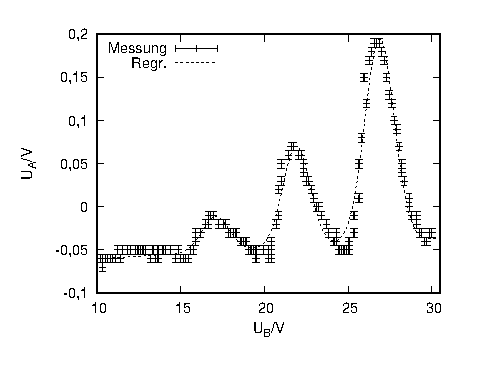
\includegraphics[width=0.7\textwidth]{data/fh/159K4V.eps}
  \caption{Anodenspannung bei $T=159^\circ$C und $U_\mathrm{G}=4$ V}
  \label{fig:159K4V}
\end{figure}


\begin{figure}[h!]
  \centering
  \begin{subfigure}[h]{0.5\textwidth}
    \centering
    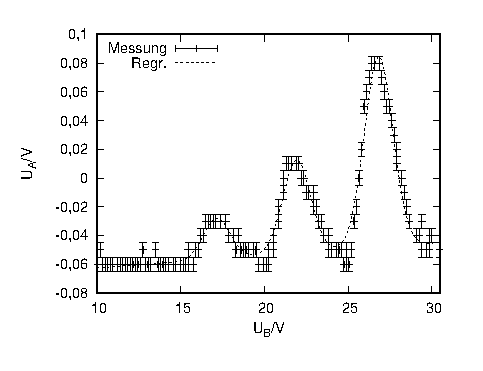
\includegraphics{data/fh/168K4V.eps}
  \end{subfigure}%
  \begin{subfigure}[h]{0.5\textwidth}
    \centering
    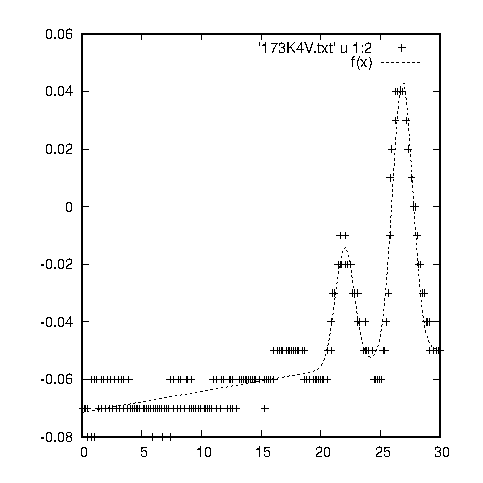
\includegraphics{data/fh/173K4V.eps}
  \end{subfigure}
    \begin{subfigure}[h]{0.5\textwidth}
    \centering
    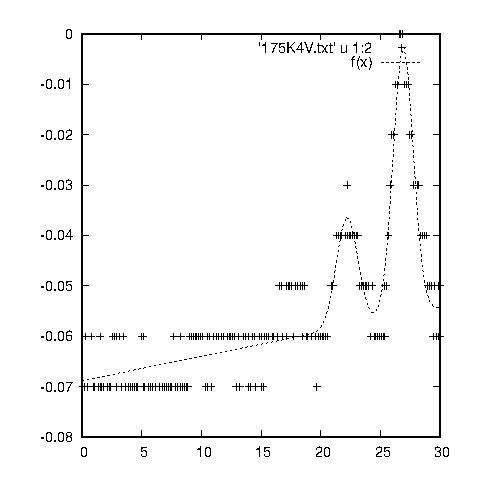
\includegraphics{data/fh/175K4V.eps}
  \end{subfigure}%
  \begin{subfigure}[h]{0.5\textwidth}
    \centering
    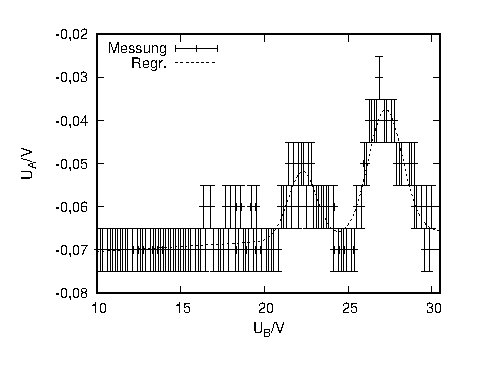
\includegraphics{data/fh/181K4V.eps}
  \end{subfigure}
  \caption{Anodenspannung für weitere Temperaturen}
  \label{fig:kennlinien1}
\end{figure}

\begin{figure}[h!]
  \centering
  \begin{subfigure}[h]{0.5\textwidth}
    \centering
    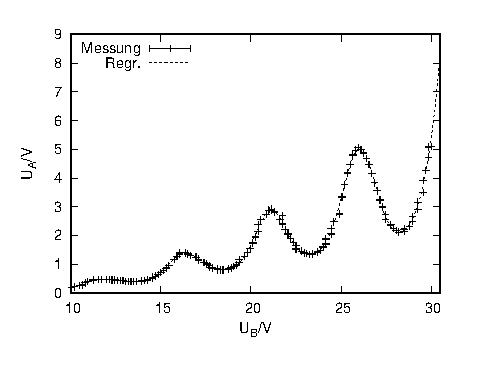
\includegraphics{data/fh/165K1V.eps}
  \end{subfigure}%
  \begin{subfigure}[h]{0.5\textwidth}
    \centering
    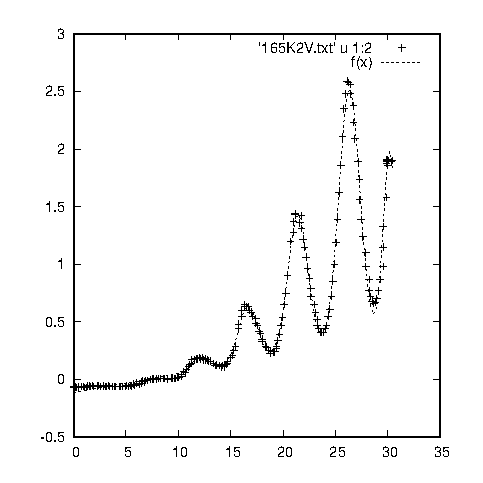
\includegraphics{data/fh/165K2V.eps}
  \end{subfigure}
    \begin{subfigure}[h]{0.5\textwidth}
    \centering
    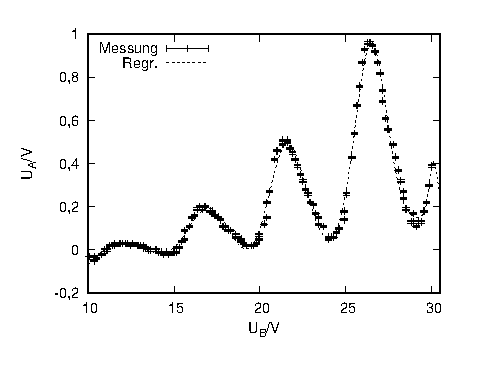
\includegraphics{data/fh/165K3V.eps}
  \end{subfigure}%
  \begin{subfigure}[h]{0.5\textwidth}
    \centering
    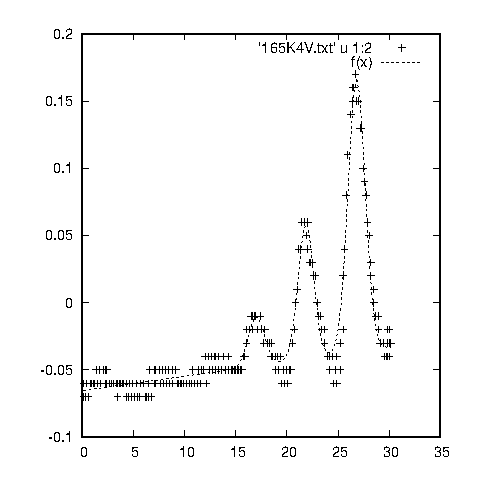
\includegraphics{data/fh/165K4V.eps}
  \end{subfigure}
  \caption{Anodenspannung für verschiedene Gegenspannungen bei $165^\circ$ C}
  \label{fig:kennlinien2}
\end{figure}


  \begin{table}[h]
    \centering
    \begin{tabular}{c | r p{0.05cm} l r p{0.05cm} l r p{0.05cm} l r p{0.05cm} l}
      \toprule
       $U_\mathrm{G}/$V & & 1 & & & 2 & & & 3 & & & 4 &\\  
      \midrule
      $U_0/$V &              -1,1         &$\pm$ & 0,1      &   -0,9        &$\pm$ & 0,1     & -0,7  & $\pm$ &  0,1  &  -0,062  & $\pm$  & 0,004 \\    
      $\alpha$ & 0,101         &$\pm$ & 0,006    &  0,052        &$\pm$ & 0,005    & 0,03  & $\pm$ & 0,005   &   0,0007 & $\pm$  & 0,002 \\
      $A_1$/V &              0,38         &$\pm$ & 0,06     &   0,45          &$\pm$ & 0,07    & 0,41  & $\pm$ &  0,09  &    &   &  \\ 
      $A_2$/V &              0,82         &$\pm$ & 0,03     &   0,63         &$\pm$ & 0,03    &  0,36 & $\pm$ & 0,04   &  0,039  & $\pm$  & 0,005 \\ 
      $A_3$/V &             1,85          &$\pm$ & 0,02     &   1,21          &$\pm$ & 0,03    & 0,58  & $\pm$ & 0,03   &  0,104  & $\pm$  & 0,005 \\ 
      $A_4$/V &              3,49          &$\pm$ & 0,04     &   2,09          &$\pm$ & 0,02    & 0,9  & $\pm$ &  0,02  &  0,208  & $\pm$  & 0,005 \\ 
      $A_5$/V &              41          &$\pm$ & 83       &   1,6          &$\pm$ & 0,6     & 0,2  & $\pm$ & 0,1   &    &  &  \\ 
      $\mu_1/$V &            11,38          &$\pm$ & 0,08     &   11,6            &$\pm$ & 0,1     & 11,4  & $\pm$ & 0,2   &    &   &  \\ 
      $\mu_2/$V &           16,29          &$\pm$ & 0,02     &  16,64          &$\pm$ & 0,04    &  17,01 & $\pm$ & 0,09   &  17  & $\pm$  & 0,1 \\ 
      $\mu_3/$V &            21,11           &$\pm$ & 0,01      &   21,34           &$\pm$ & 0,02     & 21,58  & $\pm$ & 0,02   &   21,88 & $\pm$  & 0,04 \\ 
      $\mu_4/$V &            26,01          &$\pm$ & 0,01    &   26,28          &$\pm$ & 0,01   & 26,47  & $\pm$ & 0,02   &  26,83  & $\pm$ & 0,02 \\ 
      $\mu_5/$V &            34          &$\pm$ & 2       &   30,5          &$\pm$ & 0,4     & 30,1  & $\pm$ &  0,3  &    &  &  \\ 
      $\sigma_1$/V &         1,4          &$\pm$ & 0,2      &   2,1          &$\pm$ & 0,2     & 2,8  & $\pm$ & 0,4   &    &   &  \\ 
      $\sigma_2$/V &         0,87         &$\pm$ & 0,04     &   1,08          &$\pm$ & 0,05    & 1,34  & $\pm$ &  0,09  &  0,8  & $\pm$  & 0,1 \\ 
      $\sigma_3$/V &         0,82         &$\pm$ & 0,01      &   0,94         &$\pm$ & 0,03    & 1,07  & $\pm$ & 0,06   &   0,79 & $\pm$  & 0,05 \\ 
      $\sigma_4$/V &        0,9          &$\pm$ & 0,01    &   0,89         &$\pm$ & 0,02    &  0,91 & $\pm$ &  0,02  &  0,86  & $\pm$  & 0,03 \\ 
      $\sigma_5$/V &         1,7          &$\pm$ & 0,5      &   0,6         &$\pm$ & 0,1     & 0,2  & $\pm$ & 0,1   &    &   &  \\ 
      \bottomrule
    \end{tabular}
    \caption{Parameter der Regressionskurven}
    \label{tab:fh_parameter_1}
  \end{table}

 \begin{table}[h]
    \centering
    \begin{tabular}{c | r p{0.05cm} l r p{0.05cm} l r p{0.05cm} l r p{0.05cm} l r p{0.05cm} l}
      \toprule
       $T/^\circ$C & & 159 & & & 168 & & & 173 & & & 175 & & & 181& \\  
      \midrule
      $U_0/$V &              -0,072         &$\pm$ & 0,005      &   -0,071        &$\pm$ & 0,002     & -0,072  & $\pm$ &  0,003  &  -0,068  & $\pm$  & 0,002 & -0,073 & $\pm$ & 0,002\\    
      $\alpha$& 0,0012         &$\pm$ & 0,0003    &  0,0009        &$\pm$ & 0,0001    & 0,0008  & $\pm$ & 0,0001   &   0,0005 & $\pm$  & 0,0001 & 0,0002 & $\pm$ & 0,0001\\
      $A_2$/V &              0,041         &$\pm$ & 0,005     &   0,029          &$\pm$ & 0,003    &   &  &   &    &   &  & & &\\ 
      $A_3$/V &              0,117         &$\pm$ & 0,006     &   0,065         &$\pm$ & 0,003    &  0,041 & $\pm$ & 0,003   &  0,021  & $\pm$  & 0,002 & 0,016 & $\pm$ & 0,002\\ 
      $A_4$/V &              0,237          &$\pm$ & 0,006     &   0,133          &$\pm$ & 0,003    & 0,095  & $\pm$ & 0,003   &  0,052  & $\pm$  & 0,002 & 0,029 & $\pm$ & 0,002\\ 
      $\mu_2/$V &            17,1          &$\pm$ & 0,1     &   17,16            &$\pm$ & 0,09     &   &  &    &   &   & & & &\\ 
      $\mu_3/$V &            21,91          &$\pm$ & 0,04     &   21,93          &$\pm$ & 0,04    &  21,99 & $\pm$ & 0,06   &  22,2  & $\pm$  & 0,1 & 22,27 & $\pm$ & 0,09\\ 
      $\mu_4/$V &            26,87,           &$\pm$ & 0,02      &   26,82           &$\pm$ & 0,02     & 26,83  & $\pm$ & 0,03   &   26,89 & $\pm$  & 0,04 & 27,23 & $\pm$ & 0,06\\ 
      $\sigma_2$/V &         0,8          &$\pm$ & 0,1      &   0,8          &$\pm$ & 0,1     &   &  &   &    &  &  &  & & \\ 
      $\sigma_3$/V &         0,87         &$\pm$ & 0,04     &   0,83          &$\pm$ & 0,04    & 0,76  & $\pm$ &  0,07  &  0,8  & $\pm$  & 0,1 & 0,8 & $\pm$ & 0,1\\ 
      $\sigma_4$/V &         0,82         &$\pm$ & 0,01      &   0,85         &$\pm$ & 0,02    & 0,83  & $\pm$ & 0,03   &   0,81 & $\pm$  & 0,05 & 1,02 & $\pm$ & 0,08\\ 
      \bottomrule
    \end{tabular}
    \caption{Parameter der Regressionskurven}
    \label{tab:fh_parameter_2}
  \end{table}

\begin{table}[h]
    \centering
    \begin{tabular}{c c c}
      \toprule
      $T/^\circ$C & $U_\mathrm{G}/$V & $\Delta \mu/$V\\
      \midrule
      165&1&$4,91\pm 0,09$\\
      &&$4,82\pm 0,03$\\
      &&$4,90 \pm 0,02$\\
      165&2&$5,1 \pm 0,1$\\
      &&$4,70 \pm 0,04$\\
      &&$4,93 \pm 0,02$\\
      165&3&$5,6 \pm 0,2$\\
      &&$4,51 \pm 0,09$\\
      &&$4,89 \pm 0,03$\\
      165&4&$4,8 \pm 0,1$\\
      &&$4,95 \pm 0,05$\\
      159&4&$4,8 \pm 0,1$\\
      &&$4,97 \pm 0,05$\\
      168&4&$4,8 \pm 0,1$\\
      &&$4,89 \pm 0,05$\\
      173&4&$4,85 \pm 0,07$\\
      175&4&$4,7 \pm 0,4$\\
      181&4&$5,00\pm 0,1$\\
      \bottomrule
    \end{tabular}
    \caption{Abstände von Spannungsmaxima}
    \label{tab:fh_dist}
  \end{table}
